\documentclass[a4paper, 11pt]{article}
\usepackage{comment} % enables the use of multi-line comments (\ifx \fi) 
\usepackage{lipsum} %This package just generates Lorem Ipsum filler text. 
\usepackage{fullpage} % changes the margin
\usepackage{amsmath,amsfonts,amsthm} % Math packages
\usepackage{graphicx}
\usepackage{enumitem}
\usepackage{media9}
\setlist{nolistsep}
\usepackage{geometry}
\usepackage{listings}

\geometry{bottom=15mm}

\begin{document}
%Header-Make sure you update this information!!!!
\noindent
\large\textbf{Reinforcement Learning} \hfill %\textbf{FirstName LastName} \\
\normalsize Exercise 0 \hfill 
\\Team: Nico Ott 4214197, Lior Fuks 4251285, Hendrik Vloet 4324249 \\
\hfill Date: \today \\
\hfill Due Date: November 9, 2017
\section{Introduction to RL}
\begin{itemize}
	\item \textbf{Model}: A model is an agent's internal representation of the environment that predicts its behavior, i.e. forecasts the environment's evolution, regarding an action of the agent.\\
	 A model may help a policy to find the best next action and it consists of 2 components:
	\begin{itemize}
		\item State-Transition model $\mathcal{P}$. It predicts the next state of the agent after executing an action. Formalized:
		\begin{flalign*}
			\mathcal{P}^a _{SS'} = \mathbb{P}  \left\lbrace S_{t+1}   = s' | S_t =s, A_t = a    \right\rbrace \\
		\end{flalign*}
		\item Reward model $\mathcal{R}^a _s$. It predicts the next expected (immediate) reward for the agent after performing some action, formalized:
		\begin{flalign*}
			\mathcal{R}^a _s = \mathbb{E} \lbrace R_{t+1} | S_t = s, A_t =a \rbrace \\
		\end{flalign*}
%		\vspace{-1.4cm}
%		\begin{figure}[hbpt!]
%		\centering
%		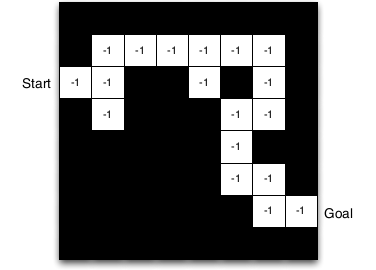
\includegraphics[width=0.5\textwidth,height=4cm]{example_model}
%		\caption{Example for a model. The grid layout represents the transition model(which can be imperfect; compare to the full grid in D.Silvers lecture) $\mathcal{P}^a _{ss'}$ and the numbers represent the immediate reward $\mathcal{R}^a _s$ from each state $s$ (in this case the same for every action $a$). Picture taken from David Silvers Reinforcement Learning Lecture.}
%		\end{figure}
	\end{itemize}
    \item \textbf{Policy}: the policy is the behavior of the agent, i.e. it is a mapping function from state to an action. Or in other words: it is a strategy how the agent will choose its next action, taking into account in which state it is. Nevertheless, a policy does not guarantee optimal performance, since it just represents one possible behavior of the agent out of infinitely many. Briefly, it can be good or bad and thus increase or decrease performance.\\
     We can divide them into two overall classes:
    \begin{itemize}
    	\item deterministic policy, where the outcome of an evaluation of the state is exactly known: \\ 
    	\begin{align*}
    	a = \pi(s)
    	\end{align*}
    	\item stochastic policy, where the outcome of an evaluation of the state is not exactly known but can be described with the help of probabilistic calculus:\\
    	\begin{align*}
    		\pi( a | s) = \mathbb{P}(A_t =a | S_t = s)
    	\end{align*}
    \end{itemize}
    \vspace{0.5cm}
    \item \textbf{Value-function}: predicts the future reward of the agent and is used to evaluate the goodness/badness of states, i.e. the value function can be used to pick actions, depending of the outcome. The value functions "unrolls" future possible rewards under some policy $\pi$. Usually, the value function cannot predict the future with absolute certainty. Therefore, expected rewards of the future will have less influence on the value of the actual state("Myopic Evaluation"):\\
    \begin{align*}
    	v_{\pi} ^{(s)} = \mathbb{E}_{\pi} \lbrace R_{t+1}+ \gamma R_{t+2} + \gamma ^2 R_{t+3}+... | S_t = s \rbrace
    \end{align*}
\end{itemize}
\clearpage


\section{GYM: 2 Versions}


We decided to design two different codings. We will describe both versions in the following. We highly encourage you to try both versions. Both should fulfill the given task description.

\subsection{Version 1: Explore and Exploit}

\textbf{File name:} ex00\_explore\_exploit.py\\
This program consists of two parts:
\begin{itemize}
	\item Exploration: Finding a good parameter set with random search
	\item Exploitation: Using the found parameter set on a few episodes to check the parameter set
\end{itemize}

\paragraph{Exploration}

In every episode, a random weight vector is created and used until the cartpole fails or reaches a total reward of 200. (200 is the maximum possible step number, after that the done flag is set and the task is considered solved) It also saves the weight parameter set which performed best but finally returns the first parameter set which reaches a total reward of 200.
Usually, the random search finds a suited parameter set within the first 20-30 episodes.

\paragraph{Exploitation}

The found parameter set is then used again for a linear combination on 5 episodes just to see if the greedily found parameter set performs well on other starting points.
Sometimes the found parameter set will do great for all runs, sometimes it won’t solve the task in a single run.

This program was kept as simple as possible to show the basic idea of the exploration \& exploitation policy.
\clearpage

\subsection{Version 2: Random Search and Hill Climbing}

The second version uses a somewhat more detailed approach but also works with linear combinations of some weighting parameters and the observations in order to determine the next action of the agent. To estimate good parameters, the program performs a random search or hill climbing.\\
The program is also able to work in a simpler mode, similar to Version 1 but is no real learning program, since it just applies randomly chosen parameters to the cartpole environment. Briefly, the program consists of the following mechanics:
\begin{enumerate}
	\item A simple demonstration of how the cartpole will behave under a \textbf{random} policy.
	\item A more detailed analysis of two different policies:
	\begin{itemize}
		\item Random Search
		\item Hill Climbing
	\end{itemize}
\end{enumerate}


\subsubsection{Setup}

\begin{itemize}
	\item \textbf{filename}: ex00\_policy\_analysis.py
	\item ONLY WORKS WITH PYTHON2
	\item Depending on the configurations in the user interface, the execution can take a while. A configuration with 1000 RUNS and 1000 TESTRUNS and the POLICY\_ANALYSIS,SHOW\_PARAMETER, SHOW\_PLOTS, TEST\_PARAM flags set to true took approx. 10-15 minutes (results are shown in figure \ref{fig:plots}).
\end{itemize}

\subsection{User Interface}


The program is completely controllable by a few parameters and flags. The default values have been set to show a short demonstration.\\
BUT WE ENCOURAGE YOU TO PLAY WITH THE POLICY\_ANALYSIS FLAG!\\
The other parameters have following functions (refer also to figure \ref{fig:interface}):
\begin{itemize}
	\item POLICY\_ANALYSIS
	\begin{itemize}
		\item \textbf{True}: enable the full analysis program, i.e. performing a random search and hill climbing (Warning: Increases runtime)
		\item \textbf{False}: disable full analysis and just show a short demo with a randomized policy within the cartpole environment
	\end{itemize}
	\item RUNS: set the total amount of runs that are used in the different parameter searches. Increasing it beyond the default(100) may increase runtime drastically
	\item RENDER: if set true, all episodes of any cartpole interaction is rendered and thus displayed. (Warning: Can increase runtime drastically!)
	\item SHOW\_PARAMETERS: if true, the program will display several additional information about used weights, rewards, observations etc. (Warning: activating it, may result in a blown up output display)
	\item NOISE\_SCALING: affects the Hill Climbing search, which uses noise injection in order to escape local minima. The higher it is, the more the Hill Climbing behaves like pure Random Search
	\item TESTRUNS: sets the amount of testruns, hat will be used to find the best parameter pairs, that have been found by Random Search and Hill Climbing
	\item SHOW\_PLOTS: if set true, several plots will show up in the end, regarding some statistics of the Random Search and the Hill Climbing (Histogram, ECDF, Success-Rate, see figure \ref{fig:plots})
	\item TEST\_PARAM: in case POLICY\_ANALYSIS and TESTRUNS is set to true, the program will try to find the best parameter pairs, which have been found by Random Search and Hill Climbing
\end{itemize}

\begin{figure}[hbpt!]
 \centering
 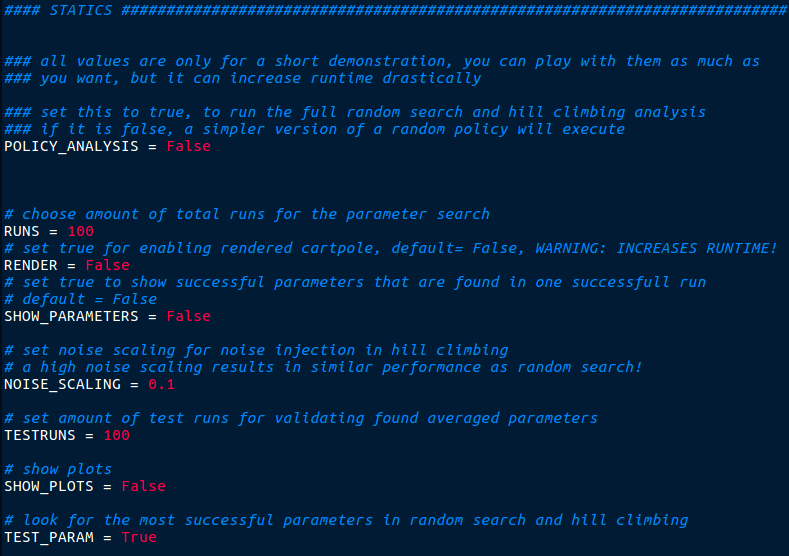
\includegraphics[width=0.8\textwidth]{interface}
 \caption{Screenshot of the user configuration part of the program}
 \label{fig:interface}
\end{figure}

\begin{figure}[hbpt!]
	\centering
	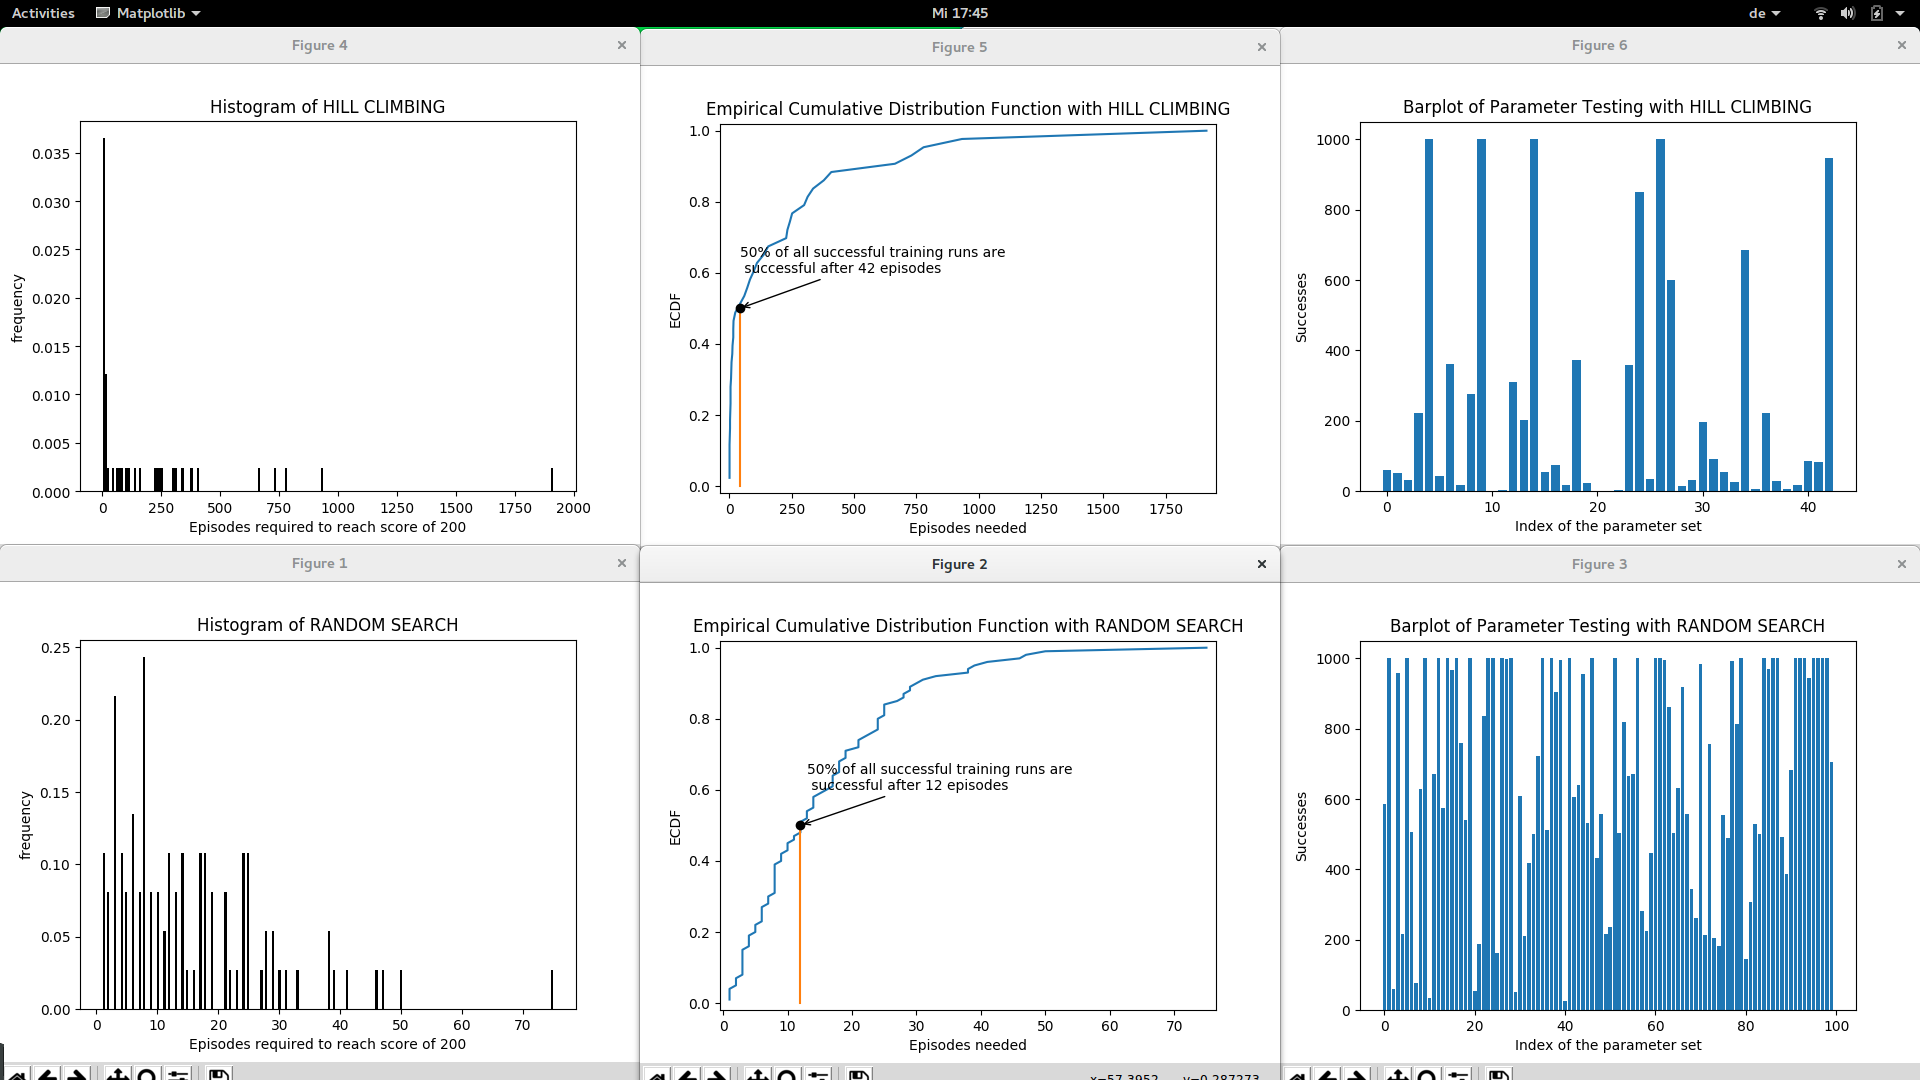
\includegraphics[width=\textwidth, height=0.75\textwidth]{1000_runs}
	\caption{Plotting results of a detailed policy analysis.}
	\label{fig:plots}
\end{figure}








\end{document}
